%%%%%%%%%%%%%%%%%%%%%%%%%%%%%%%%%%%%%%%%%%%%%%%%%%%%%%%%%%%%%%%%%
% MUW Presentation
% LaTeX Template
% Version 1.0 (27/12/2016)
%
% License:
% CC BY-NC-SA 4.0 (http://creativecommons.org/licenses/by-nc-sa/3.0/)
%
% Created by:
% Nicolas Ballarini, CeMSIIS, Medical University of Vienna
% nicoballarini@gmail.com
% http://statistics.msi.meduniwien.ac.at/
%
% Customized for UAH by:
% David F. Barrero, Departamento de Automática, UAH
%%%%%%%%%%%%%%%%%%%%%%%%%%%%%%%%%%%%%%%%%%%%%%%%%%%%%%%%%%%%%%%%%

\documentclass[10pt,compress]{beamer} % Change 10pt to make fonts of a different size
\mode<presentation>

\usepackage[spanish]{babel}
\usepackage{fontspec}
\usepackage{tikz}
\usepackage{etoolbox}
\usepackage{xcolor}
\usepackage{xstring}
\usepackage{listings}

\usetheme{UAH}
\usecolortheme{UAH}
\setbeamertemplate{navigation symbols}{} 
\setbeamertemplate{caption}[numbered]

%%%%%%%%%%%%%%%%%%%%%%%%%%%%%%%%%%%%%%%%%%%%%%%%%%%%%%%%%%%%%%%%%
%% Presentation Info
\title[Python crash course]{Python crash course}
\author{\asignatura\\\carrera}
\institute{}
\date{Departamento de Automática}
%%%%%%%%%%%%%%%%%%%%%%%%%%%%%%%%%%%%%%%%%%%%%%%%%%%%%%%%%%%%%%%%%


%%%%%%%%%%%%%%%%%%%%%%%%%%%%%%%%%%%%%%%%%%%%%%%%%%%%%%%%%%%%%%%%%
%% Descomentar para habilitar barra de navegación superior
\setNavigation
%%%%%%%%%%%%%%%%%%%%%%%%%%%%%%%%%%%%%%%%%%%%%%%%%%%%%%%%%%%%%%%%%

%%%%%%%%%%%%%%%%%%%%%%%%%%%%%%%%%%%%%%%%%%%%%%%%%%%%%%%%%%%%%%%%%
%% Configuración de logotipos en portada
%% Opacidad de los logotipos
\newcommand{\opacidad}{1}
%% Descomentar para habilitar logotipo en pié de página de portada
\renewcommand{\logoUno}{Images/isg.png}
%% Descomentar para habilitar logotipo en pié de página de portada
%\renewcommand{\logoDos}{Images/CCLogo.png}
%% Descomentar para habilitar logotipo en pié de página de portada
%\renewcommand{\logoTres}{Images/ALogo.png}
%% Descomentar para habilitar logotipo en pié de página de portada
%\renewcommand{\logoCuatro}{Images/ELogo.png}
%%%%%%%%%%%%%%%%%%%%%%%%%%%%%%%%%%%%%%%%%%%%%%%%%%%%%%%%%%%%%%%%%

%%%%%%%%%%%%%%%%%%%%%%%%%%%%%%%%%%%%%%%%%%%%%%%%%%%%%%%%%%%%%%%%%
%% FOOTLINE
%% Comment/Uncomment the following blocks to modify the footline
%% content in the body slides. 


%% Option A: Title and institute
\footlineA
%% Option B: Author and institute
%\footlineB
%% Option C: Title, Author and institute
%\footlineC
%%%%%%%%%%%%%%%%%%%%%%%%%%%%%%%%%%%%%%%%%%%%%%%%%%%%%%%%%%%%%%%%%

\begin{document}

%%%%%%%%%%%%%%%%%%%%%%%%%%%%%%%%%%%%%%%%%%%%%%%%%%%%%%%%%%%%%%%%%
% Use this block for a blue title slide with modified footline
{\titlepageBlue
    \begin{frame}
        \titlepage
    \end{frame}
}

\institute{\asignatura}

\begin{frame}[plain]{}
	\begin{block}{Objectives}
		\begin{enumerate}
		\item Overview the Python syntax
		\item Being able to program na\"ive Python scripts
		\end{enumerate}
	\end{block}

	\begin{block}{Bibliography}
        \href{https://docs.python.org/3/tutorial/}{The Python Tutorial}
	\end{block}
\end{frame}

{
\disableNavigation{white}
\begin{frame}[shrink]{Table of Contents}
 \frametitle{Table of Contents}
     \begin{columns}[t]
        \begin{column}{.5\textwidth}
            \tableofcontents[sections={1-3}]
        \end{column}
        \begin{column}{.5\textwidth}
            \tableofcontents[sections={4-7}]
        \end{column}
    \end{columns}
  % You might wish to add the option [pausesections]
\end{frame}
}

\section{Introduction}
\subsection{What is Python?}

\begin{frame}{Introduction}{What is Python? (I)}
    \begin{columns}
 	   \column{.70\textwidth}
			Python is a general-purpose, high-level, interpreted programming language
				\begin{itemize}
				\item \textit{General-purpose}: Many applications.
				\item \textit{High-level}: Abstract data structures, doing more with less code.
				\item \textit{Interpreted}: No need to compile.
				\end{itemize}

 	   \column{.30\textwidth}

	        \centering \includegraphics[width=\linewidth]{figs/python.png}
	\end{columns}
	\bigskip
			It emphasizes code \textbf{readibility} and programmer's productivity\\
\end{frame}

\begin{frame}[plain]{Introduction}{What is Python? (II)}
\centering \textit{Hello world!} examples
    \begin{columns}
 	   \column{.50\textwidth}
		\vspace{-0.2cm}
		\begin{block}{Python}
		\vspace{-0.2cm}
			\lstinputlisting{code/hello.py}
		\end{block}

		\vspace{-0.2cm}
		\begin{block}{Java}
		\vspace{-0.2cm}
			\lstinputlisting[language=java,basicstyle=\scriptsize]{code/hello.java}
		\end{block}
 	   \column{.50\textwidth}

		\vspace{-0.2cm}
		\begin{block}{C}
		\vspace{-0.2cm}
			\lstinputlisting[language=c,basicstyle=\scriptsize]{code/hello.c}
		\end{block}

		\vspace{-0.2cm}
		\begin{block}{C++}
		\vspace{-0.2cm}
			\lstinputlisting{code/hello.cpp}
		\end{block}
	\end{columns}

\end{frame}

\subsection{History}
\begin{frame}{Introduction}{History}
    \begin{columns}
 	   \column{.70\textwidth}
			\begin{itemize}
				\item Python was created by Guido van Rossum in the Netherlands
				\item \textit{Python 2.0}: Released on 2000
				\item \textit{Python 3.0}: Released on 2008. Backwards-incompatible
			\end{itemize}
			\bigskip
		\centering Python 3.X is the present but Python 2.x still popular
 	   \column{.30\textwidth}
		\centering \includegraphics[width=\linewidth]{figs/guido.jpg}
	\end{columns}
\end{frame}

\subsection{Installation}
\begin{frame}{Introduction}{Installation}
\vspace{-0,3cm}
	\begin{itemize}
		\item If you have a good OS such as Linux or Mac, you already have Python!
		\item Otherwise (Windows), you have to install it
			\begin{itemize}
			\item Visit \url{https://www.python.org/downloads/}
			\end{itemize}
		\item Bad news: There is no ``standard'' IDE
			\begin{itemize}
			\item PyCharm, Komodo, PyDev, ...
			\item \url{http://wiki.python.org/moin/PythonEditors}
            \item \textit{Notebooks} are also very popular, particularly in AI
			\end{itemize}
	\end{itemize}
    \begin{columns}
 	   \column{.40\textwidth}
		\includegraphics[width=\linewidth]{figs/pycharm.png}\\\centering PyCharm
 	   \column{.35\textwidth}
		\includegraphics[width=\linewidth]{figs/komodo.png}\\\centering Komodo
 	   \column{.3\textwidth}
		\includegraphics[width=\linewidth]{figs/pydev.png}\\\centering PyDev
	\end{columns}
\end{frame}

\subsection{The Python interpreter}

\begin{frame}{The Python interpreter}{Python operation modes}
		Python is an interpreted language, i.e., it needs an interpreter.
			\begin{itemize}
				\item Interpreted = it is not complied = it needs no compilation.
				\item Faster development, slower execution.
			\end{itemize}
		Two operation modes:
			\begin{itemize}
				\item \textbf{Interactive}: The interpreter reads the program from the \textit{stdin} (usually the keyboard).
				\item \textbf{Non-interactive}: The interpreter reads the program from a file (also known as \alert{script}).
			\end{itemize}
\end{frame}

\begin{frame}{The Python interpreter}{Interactive}
		Just run \texttt{python}
			\begin{itemize}
				\item Different names for different versions to avoid conflicts.
				\item \texttt{python}, \texttt{python3.4}, ...
			\end{itemize}

		\vspace{-0.2cm}
		\begin{exampleblock}{}
		\vspace{-0.2cm}
			\lstinputlisting[basicstyle=\scriptsize]{code/interprete.txt}
		\end{exampleblock}
		The programmer executes as he writes code down.
\end{frame}

\begin{frame}[fragile]{The Python interpreter}{Non-interactive}
	The program is in a plain text file.
		\begin{itemize}
		\item It can be edited with any text editor.
		\item Extension ``.py''.
		\item Execution permission (\texttt{chmod u+x myscript.py}).
		\item By default, UTF-8 encoding.
		\end{itemize}
	The first line must be \texttt{\#!/usr/bin/python}
		\begin{itemize}
		\item It is the interpreter location.
		\item If not present, the interpreted must be invoked.
		\end{itemize}

    \begin{columns}
 	   \column{.50\textwidth}
	
		\vspace{-0.2cm}
		\begin{exampleblock}{script.py}
		\vspace{-0.2cm}
			\lstinputlisting{code/script.py}
		\end{exampleblock}

 	   \column{.50\textwidth}
    	\begin{exampleblock}{}
\begin{verbatim}
python script.py
./script.py
\end{verbatim}
		\end{exampleblock}
	\end{columns}
\end{frame}

\section{Variables}
\subsection{Numbers}

\begin{frame}[fragile]{Variables}{Numbers (I)}
 	\textbf{Variable}: A name that refers a value.
	\begin{itemize}
		\item No need to declare variables (Python is weakly typed!).
		\item Python automatically assigns types.
		\item Basic types: Numbers, strings and booleans.
	\end{itemize}
	\textbf{Complex data structures}:
		\begin{itemize}
		\item Lists, tuples, dictionaries, associative arrays.
		\end{itemize}

    \begin{columns}
 	   \column{.40\textwidth}
	\begin{block}{Variables}
	\begin{verbatim}
variable = value
\end{verbatim}
	\end{block}
	\end{columns}
\end{frame}

\begin{frame}[fragile]{Variables}{Numbers (II)}
   	\begin{columns}
   	\column{.40\textwidth}
		\begin{exampleblock}{}
		\begin{verbatim}
>> numberA = 4
>> numberB = 2.3
>> numberA + numberB
6.3
>> string = "Spam"
>> boolean = True
>> a = b = c = 0
>> b
0
>>> type(numberA)
<type 'int'>
\end{verbatim}
		\end{exampleblock}

   	\column{.60\textwidth}

		\begin{exampleblock}{}
		\lstinputlisting{code/operdemo.py}
		\end{exampleblock}

	    \bigskip
        New Python elements:
        \begin{itemize}
            \item The \texttt{input()} function.
		    \item The \texttt{int()} and \texttt{float()} functions.
            \item The \texttt{type()} function.
        \end{itemize}
   \end{columns}
\end{frame}

\subsection{Strings}

\begin{frame}[fragile]{An informal introduction}{Strings (I)}
	Of course, variables can contain strings.
	\begin{exampleblock}{}
		\begin{verbatim}
>>> text = "hello"
>>> text = 'hello'
>>> print(text)
hello
\end{verbatim}
	\end{exampleblock}

	\begin{columns}[T]
 	   			\column{.40\textwidth}
		Strings contatenation
				\begin{exampleblock}{}
				\begin{verbatim}
>>> "hello" + " there"
'hello there'
>>> "hello" "there"
'hellothere'
\end{verbatim}
				\end{exampleblock}

 	   			\column{.30\textwidth}
		Variables with strings
				\begin{exampleblock}{}
				\begin{verbatim}
>>> a = "hello"
>>> b = " there"
>>> a + b
'hello there'
\end{verbatim}
				\end{exampleblock}

 	   			\column{.30\textwidth}
		String length
				\begin{exampleblock}{}
				\begin{verbatim}
>>> len("hello")
5
\end{verbatim}
				\end{exampleblock}
		\end{columns}
\end{frame}

\begin{frame}[fragile]{An informal introduction}{Strings (II)}
	\vspace{-0.2cm}
	F-strings: From Python 3.6
	\vspace{-0.3cm}
	\begin{columns}
\column{.70\textwidth}
\begin{block}{}
\begin{verbatim}
>>> name = 'John'
>>> age = 22
>>> print(f"Hi {name}, you are {age}")
'Hi John, you are 22'
\end{verbatim}
\end{block}
\end{columns}
\end{frame}

\begin{frame}[fragile]{An informal introduction}{Strings (III)}
	\vspace{-0.3cm}
	\begin{columns}
 		\column{.60\textwidth}
	        Strings are a sequence of characters: \alert{Slice notation}.
	        \begin{itemize}
	            \item Quite common in Python data structures.
	            \item It uses indices (as an array). First index is $0$.
	        \end{itemize}

            \begin{block}{Slice notation}
                variable[start:stop:step]
            \end{block}

   	    \column{.40\textwidth}
			\begin{exampleblock}{}
            \vspace{-0.3cm}
		    \begin{verbatim}
>>> a = "hello"
>>> a[2]
'l'
>>> a[2:]
'llo'
>>> a[:2]
'he'
>>> a[2:] + a[:2]
'llohe'
>>> a[2:4]
'll'
>>> a[::2]
'hlo'
>>> a[::-1]
'olleh'
\end{verbatim}
            \vspace{-0.2cm}
				\end{exampleblock}
		\end{columns}
\end{frame}


\subsection{Lists}
\begin{frame}[fragile]{An informal introduction}{Lists (I)}
	\textbf{List}: An ordered collection of mutable data.
	\begin{itemize}
		\item Very powerful data structure, similar to an array.
		\item \textit{Ordered}: Data in the list have a location.
		\item \textit{Mutable}: Data can be modified.
		\item Data types can be different.
	\end{itemize}
	\begin{columns}
   		\column{.70\textwidth}
		\begin{block}{List initialization}
		\begin{verbatim}
variable = [data1, data2, ..., dataN]
\end{verbatim}
		\end{block}
	\end{columns}
\end{frame}

\begin{frame}[fragile]{An informal introduction}{Lists (II)}
    \vspace{-0.7cm}
	\begin{columns}
 	   	\column{.30\textwidth}
		Initialization

   		\column{.70\textwidth}
		\begin{exampleblock}{}
		\begin{verbatim}
>>> a = ['spam', 'eggs', 123]
['spam', 'eggs', 123]
\end{verbatim}
		\end{exampleblock}
	\end{columns}

	\begin{columns}
 	   	\column{.30\textwidth}
		Slice notation, \texttt{len()} and $+$ work on lists

   		\column{.70\textwidth}
		\begin{exampleblock}{}
		\begin{verbatim}
>>> a[2]
123
>>> a[1:]
['eggs', 123]
>>> a + a
['spam', 'eggs', 123, 'spam', 'eggs', 123]
>>> len(a)
3
\end{verbatim}
		\end{exampleblock}
	\end{columns}
\end{frame}

\begin{frame}[fragile,shrink]{Data structures in Python}{Lists (III)}
    \begin{columns}
 	   \column{.40\textwidth}
	   Lists are objects: they have methods
	\begin{itemize}
		\item \texttt{list.append(x)}
		\item \texttt{list.insert(i, x)}
		\item \texttt{list.remove(x)}
		\item \texttt{list.pop()}
		\item \texttt{list.index(x)}
		\item \texttt{list.count(x)}
		\item \texttt{list.sort()}
		\item \texttt{list.reverse()}
	\end{itemize}

 	   \column{.60\textwidth}
        \scriptsize{
		\begin{exampleblock}{}
		\vspace{-0.4cm}
		\lstinputlisting{code/lists.txt}
		\vspace{-0.2cm}
		\end{exampleblock}
		}
   \end{columns}
\end{frame}

% uso de len(lista)
% uso de rodajas o slices
%\begin{frame}[shrink]{Data structures in Python}{Lists (IV)}
%Slice notation can be used in lists
%    \begin{columns}
% 	   \column{.40\textwidth}
%\scriptsize{
%		\begin{exampleblock}{}
%		\vspace{-0.4cm}
%		\lstinputlisting{code/list-slices.py}
%		\vspace{-0.2cm}
%		\end{exampleblock}
%		}
%    \end{columns}
%\end{frame}

\section{Control flow}
\subsection{Conditions}

\begin{frame}[fragile]{Control flow}{Conditions (I)}
	Conditional statements implement decision making
	\begin{itemize}
	\item Decide some code has to be executed or not.
	\item The result is a boolean.
	\item Execute code if condition is satisfied.
	\end{itemize}

	\begin{columns}
 	   	\column{.40\textwidth}
	\begin{block}{\texttt{if} statement}
		\begin{verbatim}
if <condition>:
    # Some code
else:
    # Some other code
\end{verbatim}
		\end{block}

 	   	\column{.10\textwidth}
 	   	\column{.40\textwidth}
	\begin{exampleblock}{Example}
		\begin{verbatim}
if age > 18:
    # Some code
else:
    # Some other code
\end{verbatim}
		\end{exampleblock}
	
	\end{columns}

   New Python elements:
	\begin{itemize}
	\item Comments begin with '\#'.
	\item \alert{Indentation plays a mayor role: It defines code bodies.}
	\end{itemize}
	
\end{frame}

\begin{frame}[fragile]{Control flow}{Conditions (II)}
	\begin{columns}
 	   	\column{.80\textwidth}
	\begin{exampleblock}{Nested condition}
		\begin{verbatim}
if age == 18:
    print("You are 18 years old")
elif age < 18:
    print("You are younger than 18 years old")
elif age > 18:
    print("You are older than 18 years old")
else:
    print("You should not be reading this")
\end{verbatim}
		\end{exampleblock}
	\end{columns}
	
\end{frame}


\begin{frame}[fragile]{Control flow}{Conditions (III)}
	\centering \begin{tabular}{cl|cl}\hline
	\sc Sign & \sc Operator & \sc Sign 	& \sc Operator \\ \hline
	== 	 & Equal   		& \texttt{and} 	& Logical and \\
	!= 	& Not equal  	& \texttt{or}	& Logical or  \\
	> 	& Greater 		& \texttt{not}	& Logical not \\
	< 	& Lower			&   	& \\
	>= 	& Greater or equal 		& 	& \\
	<= 	& Lower or equal 		& 	& \\\hline
	\end{tabular}

	\begin{columns}
 	   	\column{.80\textwidth}
	\begin{exampleblock}{Nested condition}
		\begin{verbatim}
if (age > 18) and (name == "Biggus Dickus"):
    print("Hi Biggus")
\end{verbatim}
		\end{exampleblock}
	\end{columns}
\end{frame}

\subsection{for Statements}
\begin{frame}{Control flow}{\texttt{for} statements (I)}
	\begin{itemize}
		\item Sometimes we have to repeat a task: Loops
			\begin{itemize}
			\item Other languages iterate over a condition
			\item For instance, in C: \texttt{for (i=0; i<10; i++)}
			\end{itemize}
		\item Two loop statements in python: \texttt{while} and \texttt{for}
		\item In Python, for iterates over a sequence (lists or strings)
			\begin{itemize}
			\item In each iteration, it assigns a sequence value to a variable
			\end{itemize}
	\end{itemize}

    \begin{columns}
    \column{.60\textwidth}
		\begin{exampleblock}{for statement example}
		\lstinputlisting{code/for.py}
		\end{exampleblock}

    \column{.40\textwidth}
		\begin{exampleblock}{for statement example}
		\lstinputlisting{code/for-string.py}
		\end{exampleblock}
	\end{columns}
\end{frame}

\begin{frame}{Control flow}{\texttt{for} statements (II)}
	Sometimes, we need to iterate over a sequence of numbers
	\begin{itemize}
		\item \texttt{range(n)}: It returns a sequence $0$, ..., $n-1$
	\end{itemize}

    \begin{columns}
    \column{.50\textwidth}
		\begin{exampleblock}{\texttt{range()} example}
		\lstinputlisting{code/for-range.py}
		\end{exampleblock}
		
    \column{.50\textwidth}
		\begin{exampleblock}{Alternative notation}
		\lstinputlisting{code/for-range2.py}
		\end{exampleblock}
	\end{columns}
\end{frame}

\begin{frame}{Control flow}{\texttt{for} statements (III)}
	List comprehensions are a concise way to create lists
	\begin{itemize}
		\item Widely used and convenient
        \item It does not return a list!
	\end{itemize}

    \begin{columns}
    \column{.40\textwidth}
		\begin{exampleblock}{List with squares}
		\lstinputlisting{code/for-square.py}
		\end{exampleblock}
		
    \column{.60\textwidth}
		\begin{exampleblock}{Alternative notation}
		\lstinputlisting{code/for-square-comprehension.py}
		\end{exampleblock}
	\end{columns}

    \bigskip

    List comprehensions support conditions

    \begin{columns}
    \column{.70\textwidth}
		\begin{exampleblock}{}
		\lstinputlisting{code/for-square-comprehension-if.py}
		\end{exampleblock}
    \end{columns}
\end{frame}

\subsection{While loop}
\begin{frame}{Control flow}{While loop}
	\begin{exampleblock}{Fibonacci series}
	\vspace{-0.2cm}
		\lstinputlisting[basicstyle=\scriptsize]{code/fibo.py}
	\end{exampleblock}

    New Python elements:
	\begin{itemize}
	\item Multiple assignments
	\end{itemize}
\end{frame}


\section{Functions}

\subsection{Defining functions}
\begin{frame}{Functions}{Defining functions (I)}
    \begin{columns}
    \column{.5\textwidth}
	\textbf{Function}: A piece of code that can be used several times
		\begin{itemize}
		\item Lazy programmers are good programmers
		\item Code reuse
		\end{itemize}
    \column{.5\textwidth}
		\begin{exampleblock}{Function 1}
		\vspace{-0.2cm}
		\lstinputlisting{code/function-1.py}
		\vspace{-0.2cm}
		\end{exampleblock}
	\end{columns}

    \begin{columns}
    \column{.5\textwidth}
	Functions can be used with parameters
		\begin{itemize}
		\item Define a function before using it
		\end{itemize}

    \column{.5\textwidth}
		\begin{exampleblock}{Function 2}
		\vspace{-0.2cm}
		\lstinputlisting{code/function-2.py}
		\vspace{-0.2cm}
		\end{exampleblock}
	\end{columns}
	\bigskip
	\centering \alert{Hint: If you have to use code more than once, place it in a function}
\end{frame}

% grados farenheit y centígrados definición de funciones

\begin{frame}{Functions}{Defining functions (II)}
    A function can return a value with the keywork \alert{return}
	\begin{exampleblock}{}
	\vspace{-0.2cm}
	\lstinputlisting{code/conversion-grados.py}
	\vspace{-0.2cm}
	\end{exampleblock}
    New Python feature:
    \begin{itemize}
        \item Docstrings
    \end{itemize}
\end{frame}

\subsection{Default argument values}
\begin{frame}{Functions}{Default argument values and keyword arguments}
    \begin{columns}
    \column{0.5\textwidth}
	Python supports default arguments:
		\begin{itemize}
		\item Poweful and simple feature.
		\item Simpler (and more flexible) function calls.
		\end{itemize}
		\vspace{-0.2cm}
    \column{0.5\textwidth}
		\begin{exampleblock}{}
		\vspace{-0.2cm}
		\lstinputlisting{code/default.py}
		\vspace{-0.2cm}
		\end{exampleblock}
	\end{columns}
	Function arguments can be named:
		\begin{itemize}
		\item It overrides classic positional arguments.
		\item Positional arguments must be first.
		\end{itemize}
		\vspace{-0.2cm}
    \begin{columns}
    \column{0.4\textwidth}
		\begin{exampleblock}{}
		\vspace{-0.2cm}
		\lstinputlisting{code/keyword.py}
		\vspace{-0.2cm}
		\end{exampleblock}

	\column{0.6\textwidth}
		\begin{exampleblock}{}
		\vspace{-0.2cm}
		\lstinputlisting{code/keyword-2.py}
		\vspace{-0.2cm}
		\end{exampleblock}
	\end{columns}
\end{frame}

\section{Data structures}

\subsection{Tuples}
\begin{frame}{Data structures in Python}{Tuples}

	\textbf{Tuple}: A sequence of items, very similar to lists.
		\begin{itemize}
		\item \small However they are not the same.
		\item \small Lists are \textit{mutable}, tuples are \textit{inmutable}.
		\item \small Tuples use to contain, \textbf{usually}, heterogeneus items.
		\item \small Lists use to contain, \textbf{usually}, homogeneus items, used to iterate.
		\end{itemize}
	
	    \begin{columns}
 	   \column{.38\textwidth}
		\begin{block}{Tuple initialization}
        tuple = (item1, item2, ..., itemN)\\
        tuple = item1, item2, ..., itemN
		\end{block}

 	   \scriptsize{
		\begin{exampleblock}{Creation}
		\vspace{-0.2cm}
		\lstinputlisting{code/tuple-declaration.py}
		\vspace{-0.2cm}
		\end{exampleblock}
		}
       \vspace{4cm}
 	   \column{.62\textwidth}
 	   \scriptsize{
		\begin{exampleblock}{Manipulation}
		\vspace{-0.2cm}
		\lstinputlisting{code/tuple-manipulation.py}
		\vspace{-0.3cm}	
		\end{exampleblock}
		}
		\vspace{2.9 cm}

	\end{columns}
\end{frame}

\subsection{Sets}
\begin{frame}{Data structures in Python}{Sets}
\vspace{-0.2cm}
	\textbf{Set}: A collection of items, unordered with no duplicates.
		\begin{itemize}
		\item \small{Membership testing.}
		\item \small{Eliminating duplicate entries.}
%		\item \small{Math operations: \texttt{union()}, \texttt{intersection()} and \texttt{difference()}.}
		\end{itemize}
\vspace{-0.2cm}
    \begin{columns}
 	   \column{.45\textwidth}

		\begin{block}{Set initialization}
        set = {item1, item2, ..., itemN}
		\end{block}

% 	   \scriptsize{
%		\begin{exampleblock}{Creation (I)}
%		\vspace{-0.2cm}
		
%		\lstinputlisting{code/set-declaration.py}
%		\vspace{-0.2cm}
%		\end{exampleblock}
%		}

 	   \column{.55\textwidth}
 	  \scriptsize{
 	   \begin{exampleblock}{Creation}
		\vspace{-0.2cm}
		
		\lstinputlisting{code/set-manipulation1.py}
		\vspace{-0.2cm}
		
		\end{exampleblock}
		\vspace{0.3cm}
		}
	\end{columns}
	\vspace{0.1cm}
\small{\textbf{Sequence}: All types that behaves like sequences: Strings, lists and tuples.}
\end{frame}

%\begin{frame}{Other data structures in Python}{Sets (II)}
	

 	   %\scriptsize{
% 	   \begin{block}{Manipulation (I)}
%		\vspace{-0.2cm}
%		\lstinputlisting{code/set-manipulation.py}
%		\vspace{-0.2cm}
%		\end{block}		
	%	}
%\end{frame}		

\subsection{Dictionaries}
\begin{frame}{Data structures in Python}{Dictionaries (I)}
	\textbf{Dictionary}: A collection of pairs \texttt{<key, value>}
		\begin{itemize}
		\item Also named as \textit{associative array}, very similar to hash maps.
		\item Lists are indexed with a number, dictionaries use keys.
		\item Key: Numbers, strings, tuples and any inmutable type.
		\end{itemize}

    \begin{columns}
	    \column{.50\textwidth}

        \begin{block}{Dictionary initialization}
        dict = \{key1: value1, key2:value2\}
		\end{block}

 	    \scriptsize{
		\begin{exampleblock}{Creation}
		\vspace{-0.2cm}
		\lstinputlisting{code/dict-declaration.py}
		\vspace{-0.2cm}
		\end{exampleblock}
		\vspace{0.7cm}
        }
 	   \column{.50\textwidth}
 	    \scriptsize{
		\begin{exampleblock}{Manipulation}
		\vspace{-0.2cm}
		\lstinputlisting{code/dict-manipulation.py}
		\vspace{-0.2cm}
		\end{exampleblock}
        }
	\end{columns}
\end{frame}
% alguna cuestión más sobre su manipulación. Por ejemplo, se pueden borrar todos sus elementos con clear()
% len(dicc), dicc.has_key(k) o k in dicc, dicc.keys() como aparece en el ejemplo anterior: lista de claves, dicc.items() -los elementos como lista de pares

\begin{frame}{Data structures in Python}{Dictionaries (II)}
	Dictionaries can be iterated by key or by value
		\begin{itemize}
		\item Loop syntax is slightly different
		\item \texttt{item()} method
		\end{itemize}

    \begin{columns}
 	   \column{1.1\textwidth}
		\begin{exampleblock}{Dictionary iteration}
		\vspace{-0.2cm}
		\lstinputlisting{code/dict-iteration.py}
		\vspace{-0.2cm}
		\end{exampleblock}
	\end{columns}
\end{frame}


\subsection{Summary}
\begin{frame}{Data structures in Python}{Summary}
	
\centering \begin{tabular}{l|l}
\hline
\sc Data structure & \sc Initialization  \\\hline
List   & \texttt{li = [1, 2, 3]} \\
Tuple  & \texttt{tu = (1, 2, 3)} \\
	   & \texttt{tu = 1, 2, 3} \\
Set    & \texttt{se = \{1, 2, 3\}} \\
Dictionary& \texttt{dic = \{'abc' : 1, 'bca' : 2\}} \\\hline
\end{tabular}
\end{frame}

\section{Modules}
\subsection{Introduction}
\begin{frame}{Modules}{Introduction (I)}
		You loose everything when exit the interpreter
			\begin{itemize}
			\item \textit{Solution}: Write it down in a script
			\end{itemize}
		When a script becomes big, it is difficult to maintain
			\begin{itemize}
			\item \textit{Solution}: Split your script in several ones
			\end{itemize}
		As you get more scripts, you will need to reuse your functions
			\begin{itemize}
			\item \textit{Solution}: Create a \alert{module}
			\item \textbf{Module}: A file that contains definitions, functions and classes
			\end{itemize}
		If a module is too big, it is too difficult to maintain
			\begin{itemize}
			\item \textit{Solution}: Create a \alert{package}
			\item \textbf{Package}: A module of modules
			\end{itemize}
\end{frame}

\IfStrEq{\modo}{mcyte}{
\begin{frame}{Modules}{Introduction (II)}
    Lots of packages for space!!!
    \bigskip

    \begin{columns}
       \column{.30\textwidth}
            \centering 
\includegraphics[width=\linewidth]{figs/astropy.png}
            \href{https://www.astropy.org/}{(AstroPy)}
       \column{.30\textwidth}
            \centering 
\includegraphics[width=\linewidth]{figs/sunpy.jpg}
            \href{https://sunpy.org/}{(SunPy)}
       \column{.30\textwidth}
            \centering 
\includegraphics[width=\linewidth]{figs/spacepy.jpg}
            \href{https://github.com/spacepy/spacepy}{(SpacePy)}
    \end{columns}

    \bigskip

    \begin{columns}
       \column{.30\textwidth}
            \centering 
\includegraphics[width=\linewidth]{figs/astroml.png}
            \href{https://www.astroml.org/}{(AstroML)}
       \column{.30\textwidth}
            \centering 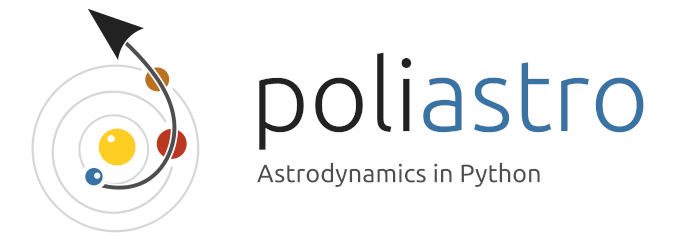
\includegraphics[width=\linewidth]{figs/poliastro.png}
            \href{https://docs.poliastro.space/en/stable/index.html}{(Poliastro)}
    \end{columns}
\end{frame}

}{}

\subsection{Installing packages}
\begin{frame}[fragile]{Modules}{Installing packages}
	Command-line automatic tool:\texttt{pip} 
		\begin{itemize}
			\item Very similar to \texttt{apt-get} in Linux
		\end{itemize}

	\begin{block}{pip usage}
	\begin{verbatim}
$ python -m pip install SomePackage
\end{verbatim}
	\end{block}

	\begin{block}{pip alternative usage}
	\begin{verbatim}
$ pip3 install SomePackage
\end{verbatim}
	\end{block}
	Example of the PIL  installation:\\
	\texttt{\$ pip3 install Pillow}\\
    \href{http://recursospython.com/guias-y-manuales/instalacion-y-utilizacion-de-pip-en-windows-linux-y-os-x/}{(More info)}
\end{frame}

\begin{frame}[fragile]{Modules}{Namespaces (I)}
    \vspace{-0.5cm}
	\begin{columns}
 	   \column{.60\textwidth}
	\begin{block}{Importing packages}
	\begin{verbatim}
import <package> [as <name>]
\end{verbatim}
	\end{block}
    \end{columns}

    \smallskip

	A module can import other modules
		\begin{itemize}
		\item Name conflicts may arise: Each module has a symbol table
		\item It means you should invoke it as \texttt{modname.itemname}
        \item The module name can be changed with the keywork \textit{as}
		\end{itemize}

	\begin{columns}
 	   \column{.40\textwidth}
	\begin{exampleblock}{}
	\begin{verbatim}
>>> import math
>>> math.log(10)
2.302585092994046
\end{verbatim}
	\end{exampleblock}

 	   \column{.40\textwidth}
	\begin{exampleblock}{}
	\begin{verbatim}
>>> import math as m
>>> m.log(10)
2.302585092994046
\end{verbatim}
	\end{exampleblock}
    \end{columns}

\end{frame}

\subsection{Namespaces}
\begin{frame}[fragile]{Modules}{Namespaces (II)}
 	It is possible to import items directly
		\begin{itemize}
		\item \texttt{from module import name1, name2}
		\item \texttt{from module import *}
		\item It uses the global symbol table (no need to use the modname)
			\end{itemize}
	
	\begin{columns}
 	   \column{.40\textwidth}
	\begin{exampleblock}{}
	\begin{verbatim}
>>> from math import log
>>> log(10)
2.302585092994046
\end{verbatim}
	\end{exampleblock}

 	   \column{.40\textwidth}
	\begin{exampleblock}{}
	\begin{verbatim}
>>> from math import *
>>> log(10)
2.302585092994046
\end{verbatim}
	\end{exampleblock}
 
    \end{columns}
\end{frame}

\subsection{Examples}

\begin{frame}{Modules}{Example 1: Open a web browser}
	\vspace{-0.2cm}
	\begin{exampleblock}{browser.py}
	\vspace{-0.2cm}
	\lstinputlisting{code/browser.py}
	\vspace{-0.2cm}
	\end{exampleblock}

    also 

	\begin{exampleblock}{browser2.py}
	\vspace{-0.2cm}
	\lstinputlisting{code/browser2.py}
	\vspace{-0.2cm}
	\end{exampleblock}

\end{frame}

\begin{frame}[plain]{Modules}{Example 2: Create a thumbnail}
	\begin{columns}
 	   \column{.60\textwidth}

		\vspace{-0.2cm}
		\begin{exampleblock}{thumbnail.py}
		\vspace{-0.2cm}
		\lstinputlisting{code/thumbnail.py}
		\vspace{-0.2cm}
		\end{exampleblock}

  		\column{.50\textwidth}
		\vspace{-0.2cm}
		\centering \includegraphics[width=\linewidth]{figs/africa.jpg}\\
	 	\texttt{africa.jpg}
	\end{columns}
		\vspace{-0.2cm}
	\centering \tiny{\href{http://www.pythonforbeginners.com/gui/how-to-use-pillow}{(Source)}}
\end{frame}

\begin{frame}{Modules}{Example 3: Plot}
	\begin{columns}
 	   \column{.60\textwidth}

		\vspace{-0.2cm}
		\begin{exampleblock}{plot.py}
		\vspace{-0.2cm}
		\lstinputlisting{code/plot.py}
		\vspace{-0.2cm}
		\end{exampleblock}

  		\column{.50\textwidth}
		\vspace{-0.2cm}
		\centering 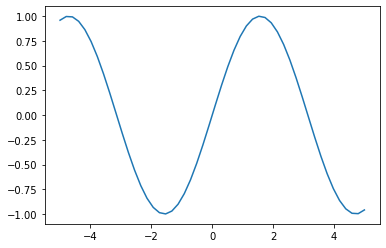
\includegraphics[width=\linewidth]{figs/plot.png}\\
	\end{columns}
		\vspace{-0.2cm}
\end{frame}

\section{Classes in Python}

\begin{frame}{Classes in Python (I)}
\vspace{-0.2cm}
\begin{itemize}			
		\item \small{\textbf{Class}: Start with the word \alert{class} followed by class name written in \alert{capital letter} and a colon [Substantives].}
		\item \small{\textbf{Attributes}: A lowercase noun.}
		\begin{itemize}
		\item \footnotesize{There is no need to declare attributes.}
		\end{itemize}
		
		\item \small{\textbf{Inherited class}: Similar to a class but the class name followed by the class father in brackets.}
		\item \small{\textbf{Instance}: Object in lower case followed by the class assignment.}
			\vspace{-0.2cm} 
  	   \begin{columns}
 	   \column{0.8\textwidth}
			\begin{block}{\small{coche.py}}
			\vspace{-0.3cm} 
				\lstinputlisting[basicstyle=\ttfamily\scriptsize]{code/coche.py} % contar elementos
				\vspace{-0.2cm} 
			\end{block}
	\end{columns}		
\end{itemize}			
\end{frame}

\begin{frame}{Classes in Python (II)}
\begin{itemize}
	\item \textbf{Method}: Start with the word \alert{def}
   \begin{itemize}
   \item Methods receive automatically a reference to the object (usually named \texttt{self}).
   \end{itemize}
		\item \textbf{Constructor}: Method whose name is \texttt{\_\_init\_\_()}, the first attribute is \texttt{self}.

		\item All methods and attributes are public.
			\begin{itemize}
				\item By convention, private members begin with double underscore (\texttt{\_\_varName}, \texttt{\_\_method\_name()})
			\end{itemize}
\end{itemize}			
\end{frame}

\begin{frame}[fragile]{Classes in Python (III)}
	\centering {Two operations on classes}
    \begin{columns}
 	   \column{.50\textwidth}
	   		\begin{block}{Instantiation}
			Creates a new object\\
			Standard functional notation\\
			\bigskip
			\centering{\texttt{x = MyClass()}}\\
	   		\end{block}
	   		\begin{exampleblock}{Example}
\begin{verbatim}
time = Time()
\end{verbatim}
	   		\end{exampleblock}
 	   \column{.50\textwidth}
	   		\begin{block}{Attribute references}
			Accesses an attribute value\\
			Standard dot syntax\\
			\bigskip
			\centering{\texttt{obj.name}}\\
	   		\end{block}
	   		\begin{exampleblock}{Example}
\begin{verbatim}
time.hour = 4
print(time.hour)
hour = time.hour
\end{verbatim}
	   		\end{exampleblock}

	\end{columns}
\end{frame}


\end{document}
